\documentclass[10pt]{beamer}

\usetheme{Warsaw}
\beamertemplatenavigationsymbolsempty

\usepackage[utf8]{inputenc}
\usepackage[T1]{fontenc}
\usepackage[francais]{babel}
\usepackage[autolanguage]{numprint}
\renewcommand*{\rmdefault}{fxb}
\usepackage{libertine}
\usepackage{lettrine}
\usepackage{hyperref}
\usepackage{wasysym}
\usepackage{listings}
\usepackage{xcolor}
\lstset{keywordstyle=\color{blue}, stringstyle=\color{green}}
\usepackage{amsmath}
\usepackage{wrapfig}
\usepackage{skak}
\usepackage{euler}
\usepackage{multicol}
\usepackage{graphicx}
\usepackage{tikz}
\usetikzlibrary{mindmap,trees}
\graphicspath{{./img/}}
\DeclareGraphicsExtensions{.png, .jpeg, .jpg}


\renewcommand*\thesection{\arabic{section}}

\AtBeginSection[]{%
  \begin{frame}<beamer>
    \frametitle{Outline}
    \tableofcontents[sectionstyle=show/hide,subsectionstyle=hide/show/hide]
  \end{frame}
  \addtocounter{framenumber}{-1}
}


\lstset{basicstyle=\footnotesize}

\title{Classification automatique de la fonction de citation}
\author{Rémi Bois et Soufian Salim}
\date{\today}

\begin{document}

\begin{frame}
  \maketitle
\end{frame}

\section{Introduction}
\label{sec:intro}

\begin{frame}
  \frametitle{L'article en question}
  %nom des auteurs, du papier, publication
\end{frame}

\begin{frame}
  \frametitle{Pourquoi citons-nous ?}
  %intérêt des citations
\end{frame}

\begin{frame}
  \frametitle{Quel rôle a une citation dans un papier ?}
  %types de citations (positives, négatives, ...)
  %différence entre fonction et motivation
\end{frame}

\begin{frame}
  \frametitle{Est-il intéressant de connaître les raisons de la
    citation ?}
  %applications au résumé, à la RI via citations, ...
  %motivations (sentiment analisys, ...)
\end{frame}

\begin{frame}
  \frametitle{Est-il possible de repérer automatiquement le type de
    citation ?}
  %Objectifs du papier, approche manuelle + apprentissage
\end{frame}


\section{Catégorisation et annotation manuelle}
\label{sec:catandmanual}


\begin{frame}
  \frametitle{Les différentes catégories}
  %tableau des catégories
\end{frame}

\begin{frame}
  \frametitle{Les données}
  %source, stats sur la taille des données
\end{frame}

\begin{frame}
  \frametitle{L'annotation manuelle des données}
  %règles, quantités, ...
\end{frame}

\begin{frame}
  \frametitle{Résultats de l'annotation manuelle}
  %Kappa, distribution, ...
\end{frame}

\section{Classification automatique}
\label{sec:machinelearning}

\begin{frame}
\frametitle{Du machine learning}
  % KPPV (3), 10-fold
  \begin{itemize} 
  \item Algorithme des 3 plus proches voisins, avec validation en 10-fold.
  \item Corpus original de 116 articles, 2829 citation, annotées manuellement.
  \end{itemize}
  \begin{figure}[h]
    \centering
    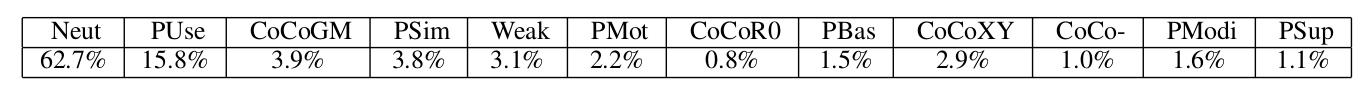
\includegraphics[width=\textwidth]{distrib}
    \caption{Distribution des citations}
  \end{figure}
\end{frame}

\begin{frame}
  \frametitle{Les features utilisées}
  Usage intensif de cue phrases
  \begin{itemize}
  \item 20 clusters de cue phrases verbales, chacune ``associée'' à un
    type de citation (eg : ``agree with'', ``be derived from'', ``be
    limited to'', ...)
  \item 12 features pour dénoter la présence de 892 cue phrases
    récupérées manuellement ($\approx 75$ par catégorie).
  \item Reconnaissance du meta-discours (``as far as we are aware'',
    ...) via une grammaire de 1762 cue phrases
  \end{itemize}
  Reconnaissance de l'agent
    \begin{itemize}
    \item 185 patterns pour reconnaître l'agent
    \item Distinction entre 2 agents : les auteurs et le reste
    \end{itemize}
  Autres features
  \begin{itemize}
  \item Mode, temps, voix
  \item localisation (globale, intra-paragraphe,
    intra-section)
  \item Auto-citation
  \end{itemize}

%cue phrases, location, ...
\end{frame}

\begin{frame}
  \frametitle{Résultats de la classification automatique}
  \begin{figure}[h]
    \centering
    \includegraphics[width=\textwidth]{resML}
    \caption{Résultats 10-fold de 3-PPV}
    \label{fig:resml12}
  \end{figure}
  %résultats sur les 12 catégories, Kappa, F-measure
\end{frame}

\begin{frame}
  \frametitle{Résultats sur des classes moins nombreuses}
  %tableaux et Kappas sur les 3/4 classes
     \begin{columns}[t]
      \begin{column}{0.5\textwidth}
        \begin{figure}[h]
          \centering
          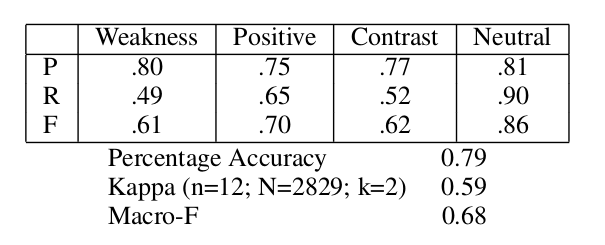
\includegraphics[width=\textwidth]{shortres4}
          \caption{Résultats sur 4 catégories}
          \label{fig:res4}
        \end{figure}
      \end{column}
      \begin{column}{0.5\textwidth}
       \begin{figure}[h]
          \centering
          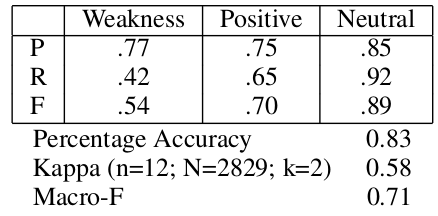
\includegraphics[width=0.75\textwidth]{shortres3}
          \caption{Résultats sur 3 catégories}
          \label{fig:res3}
        \end{figure}
      \end{column}
   \end{columns}
\end{frame}

\section{Conclusion}
\label{sec:conclusion}

\begin{frame}
  \frametitle{Des premières pistes pour une nouvelle tâche}
  \begin{itemize}
  \item Premiers résultats encourageants 
  \item Une liste de features assez importante
  \end{itemize}

  %Premiers résultats "encourageants"
\end{frame}

\begin{frame}
  \frametitle{Quelques limites présentes}
  \begin{itemize}
  \item Kappa max de 0.72 (accord inter-annotateurs) 
  \item Des features en très (trop ?) grand nombre 
  \item Une annotation manuelle très restrictive (150 règles à respecter)
  \end{itemize}
  %Kappa max de 0.72, annotation manuelle très restrictive, ...
\end{frame}

\begin{frame}
  \frametitle{Questions ?}
  \begin{figure}[h]
    \centering
    
\includegraphics[width=0.7\textwidth]{questions}
  \end{figure}
\end{frame}


\end{document}